\documentclass[11pt,a4paper]{article}
\usepackage{graphicx}
%\graphicspath{{/home/jordir/Dropbox/UdG/logos/}{../imatges/}}% Lloc on hi ha els logos

\usepackage[catalan]{babel}
\usepackage[utf8]{inputenc}
\usepackage[margin=2.5cm]{geometry}
\usepackage{graphicx}
\usepackage[x11names]{xcolor}
\usepackage{scalerel} % per escalar gràfics a mida lletres
\usepackage{hyperref}
\usepackage{nameref}
\usepackage{listings} % per codi
\usepackage{comment} % per amagar troços
\usepackage{lscape} % per posar pàgines apaisades
\usepackage{fancyhdr}
\usepackage{makecell}
\usepackage{wrapfig}
\usepackage{fontawesome}
\usepackage{pdflscape}
\usepackage{biblatex} %Imports biblatex package
\addbibresource{biblio.bib} %Import the bibliography file

\newcommand{\Cpp}{{C\texttt{++}}}
\usepackage{contour}
\definecolor{contornCobit}{RGB}{75,150,75}
\definecolor{pellCobit}{RGB}{100,200,100}
\newcommand{\cobit}{\contour{contornCobit}{\large\textcolor{pellCobit}{\textbf{CoBit10011}}}}

\pagestyle{fancy}
\lstset{language=C++}

\lhead{PdA - ViquipediaSimil, curs 2022/23 GEINF}
\rhead{\thepage}
\cfoot{}
\begin{document}
    \begin{titlepage}
        \newcommand{\HRule}{\rule{\linewidth}{0.5mm}} % Defines a new command for the horizontal lines, change thickness here
	\begin{flushleft}
            
\includegraphics[height=1.5cm]{EPS.png}\\\vfill
        \end{flushleft}
        \center % Center everything on the page
        %----------------------------------------------------------------------------------------
        %	HEADING SECTIONS
        %----------------------------------------------------------------------------------------
        \textsc{\huge \bfseries Pràctiques  - Programació declarativa. Aplicacions}\\[0.25cm]
        \textsc{\Large \bfseries Curs 2022/23}\\[0.25cm]
        \textsc{\large GEINF }
        %----------------------------------------------------------------------------------------
        %	TITLE SECTION
        %----------------------------------------------------------------------------------------
	\HRule \\[0.4cm]
        { \huge \bfseries Pràctica ViquipediaSimil} \\[0.25cm]{\Large \bfseries Angel Molero 41512839R – u1967593@campus.udg.edu}\\[0.40cm] % Title of your document
	 {\Large \bfseries Gabriel Lopez 41511387K – u1968394@campus.udg.edu}\\[0.4cm]
	 {\Large \bfseries Professor: Mateu Villaret Auselle }\\[0.4cm]

        \HRule \\\vfill
	\end{titlepage}

\tableofcontents

\clearpage

\appendix

% Secció: Introducció
\section{Introducció}

L'objectiu de la pràctica consisteix en analitzar el contingut de diversos fitxers i comprovar la seva similitud. S'ha realitzat de dues formes diferents, la primera de forma iterativa i la segona mitjançant mappers i reducers. 
Encara que l'objectiu sigui el mateix, el resultat final será diferent, ja que, a la primera s'utilitzen un número reduït de documents a analitzar, mentre que a la segona s'utilitzen 5000.

Dins el directori \textbf{primeraPart} es pot veure el codi realitzar per la primera part i un document del mateix.

% Secció: Descripció de les classes
\section{Descripció de les classes}

\begin{itemize}

	\item \textbf{Main.scala}: Dins l'objecte \textbf{Main} trobem els mètodes principals dels diferents mappers i reducers, i on s'executa el codi inicial.
	\item \textbf{InfoFicheros.scala}: Dins l'objecte \textbf{InfoFicheros} guardem aspectes dels diferents fitxers analitzats i alguns mètodes auxiliars. Així calculem alguns aspectes un únic cop i millorem el rendiment.
	\item \textbf{MapReduceActors.scala}: En aquest fitxer trobem les classes \textbf{Mapper}, \textbf{Reducer} i \textbf{MapReduce} on s'han modificat per complir amb els objectius de la pràctica.
\end{itemize}


% Secció: Extractes comentats del codi
\section{Extractes comentats del codi}

	\subsection{Primera Part}
		S'han agafat les funcions d'ordre superior més rellevants.
	
		\begin{itemize}
			\item \textbf{toFloat}: Mètode utilitzat per convertir el valor a float. Un exemple d'ús:
				\begin{center}
					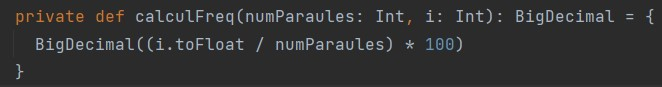
\includegraphics[height=2cm]{captures/primeraPart/ordreSuperior/toFloat.jpg}
				\end{center}
				
			\item \textbf{foldLeft}: Mètode que agafa una funció d'ordre superior i l'utilitzará per col·lapsar la col·lecció. Un exemple d'ús, per calcular la freqüència total de les paraules. Ens serveix per recorrer i guardar el valor anterior:
				\begin{center}
					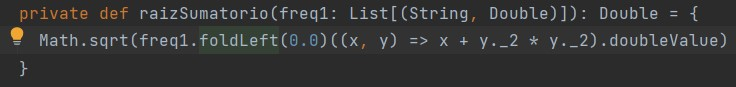
\includegraphics[height=1.8cm]{captures/primeraPart/ordreSuperior/foldLeft.jpg}
				\end{center}
				
			\item \textbf{map}: Mètode que aplica una funció a cada element de la col·lecció. L'hem utilitzat per calcular la freqüència normal. Exemple d'ús:
				\begin{center}
					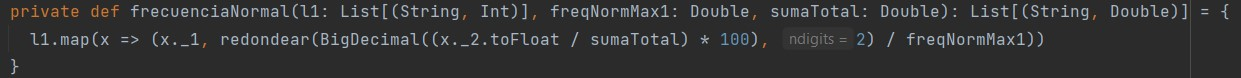
\includegraphics[height=1cm]{captures/primeraPart/ordreSuperior/map.jpg}
				\end{center}
				
			\item \textbf{setScale}: Mètode utilitzat per redondejar. Exemple d'ús:
				\begin{center}
					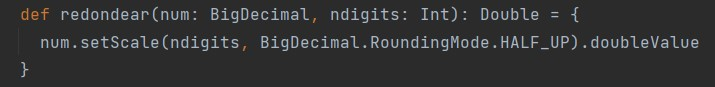
\includegraphics[height=1.5cm]{captures/primeraPart/ordreSuperior/setScale.jpg}
				\end{center}
				
			\item \textbf{compareTo}: Mètode comparar dues cadenes. L'utilitzem per saber quina de les dues cadenes hem d'avançar. Exemple d'ús:
				\begin{center}
					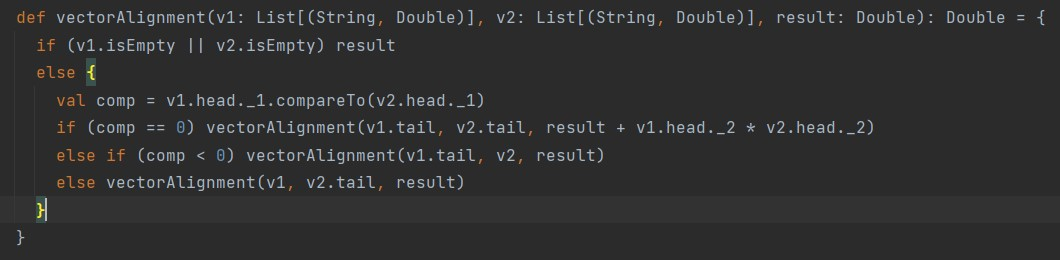
\includegraphics[height=3cm]{captures/primeraPart/ordreSuperior/compareTo.jpg}
				\end{center}
				
			\item \textbf{sliding}: Utilitzada per dividir la llista en n grames. Exemple d'ús:
				\begin{center}
					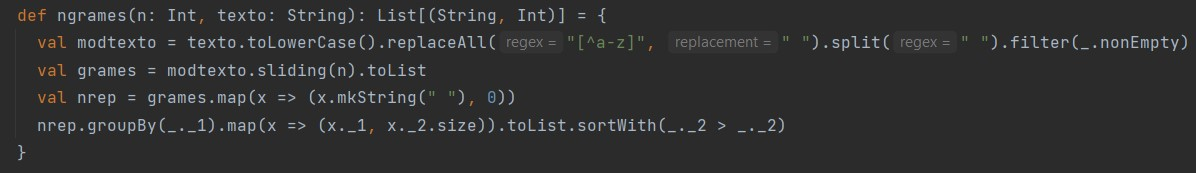
\includegraphics[height=2cm]{captures/primeraPart/ordreSuperior/sliding.jpg}
				\end{center}
				
			\item \textbf{groupBy}: Utilitza el predicat rebut per agrupar i formar un Map. L'utilizem agafant els nGrames (1 2) i formats com una cadena i els agrupem per key i així agrupem per nGrama. Exemple d'ús:
				\begin{center}
					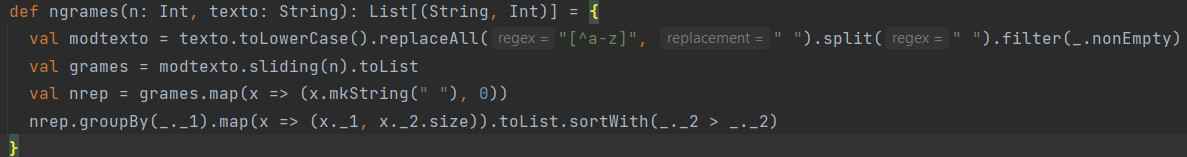
\includegraphics[height=2cm]{captures/primeraPart/ordreSuperior/groupBy.jpg}
				\end{center}
				
			\item \textbf{distinct}: Aquest mètode l'utilitzem per guardar només les paraules úniques, i així no repetir. Exemple d'ús:
				\begin{center}
					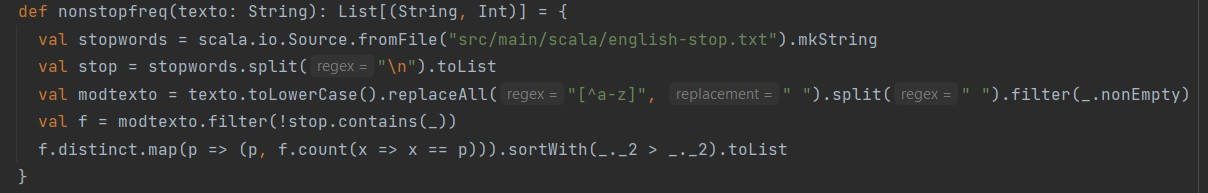
\includegraphics[height=2.5cm]{captures/primeraPart/ordreSuperior/distinct.jpg}
				\end{center}
		\end{itemize}
		
	\subsection{Segona Part}
		A la segona part no cal destacar cap funció d'ordre superior, totes les utilitzades són molt comunes.
		
		\subsubsection{Modificació MapReduce}

	

% Secció: Càlculs realitzats
\section{Càlculs realitzats}

	\begin{itemize}
		\item \textbf{input}: 
		
		\begin{itemize}
		
			\item \textbf{mappingLlegir i reduccingLlegir}:
			\begin{itemize}
				\item \textbf{K1}:
				\item \textbf{V1}:
				\item \textbf{K2}:
				\item \textbf{V2}:
				\item \textbf{V3}:
			\end{itemize}
			
			\item \textbf{mappingRef i reduccingRef}:
			\begin{itemize}
				\item \textbf{K1}:
				\item \textbf{V1}:
				\item \textbf{K2}:
				\item \textbf{V2}:
				\item \textbf{V3}:
			\end{itemize}
			
			\item \textbf{mappingCombNoRef i reduccingCombNoRef}:
			\begin{itemize}
				\item \textbf{K1}:
				\item \textbf{V1}:
				\item \textbf{K2}:
				\item \textbf{V2}:
				\item \textbf{V3}:
			\end{itemize}
			
			\item \textbf{mappingWC i reduccingWC}:
			\begin{itemize}
				\item \textbf{K1}:
				\item \textbf{V1}:
				\item \textbf{K2}:
				\item \textbf{V2}:
				\item \textbf{V3}:
			\end{itemize}
			
			\item \textbf{mappingTF i reduccingTF}:
			\begin{itemize}
				\item \textbf{K1}:
				\item \textbf{V1}:
				\item \textbf{K2}:
				\item \textbf{V2}:
				\item \textbf{V3}:
			\end{itemize}
			
			\item \textbf{mappingTfIdf i reduccingTfIdf}:
			\begin{itemize}
				\item \textbf{K1}:
				\item \textbf{V1}:
				\item \textbf{K2}:
				\item \textbf{V2}:
				\item \textbf{V3}:
			\end{itemize}
			
			\item \textbf{mappingGirar i reduccingGirar}:
			\begin{itemize}
				\item \textbf{K1}:
				\item \textbf{V1}:
				\item \textbf{K2}:
				\item \textbf{V2}:
				\item \textbf{V3}:
			\end{itemize}
			
			\item \textbf{mappingPalDoc i reduccingPalDoc}:
			\begin{itemize}
				\item \textbf{K1}:
				\item \textbf{V1}:
				\item \textbf{K2}:
				\item \textbf{V2}:
				\item \textbf{V3}:
			\end{itemize}
			
			\item \textbf{mappingRaizSumatorio i reduccingRaizSumatorio}:
			\begin{itemize}
				\item \textbf{K1}:
				\item \textbf{V1}:
				\item \textbf{K2}:
				\item \textbf{V2}:
				\item \textbf{V3}:
			\end{itemize}
			
			\item \textbf{mappingCosinoSimil i reduccingCosinoSimil}:
			\begin{itemize}
				\item \textbf{K1}:
				\item \textbf{V1}:
				\item \textbf{K2}:
				\item \textbf{V2}:
				\item \textbf{V3}:
			\end{itemize}
		\end{itemize}
		
	\end{itemize}

% Secció: Jocs de proves
\section{Jocs de proves}

	\subsection{Resultats Execucions Primera Part}
	
		\subsubsection{Freqüència de paraules}
		
			\begin{center}
				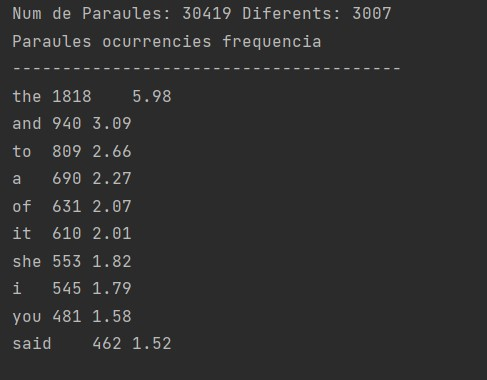
\includegraphics[height=7cm]{captures/primeraPart/freq/resultatFreq.jpg}
			\end{center}
		
		\subsubsection{Sense stop-words}
		
			\begin{center}
				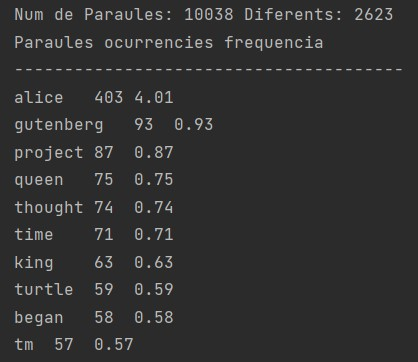
\includegraphics[height=8cm]{captures/primeraPart/sensestopwords/execucio.jpg}
			\end{center}
		
		\subsubsection{Distribució de paraules}
		
			\begin{center}
				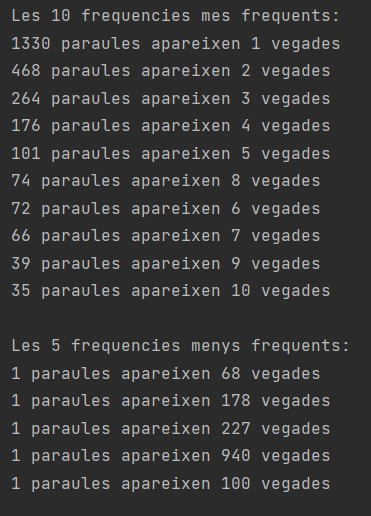
\includegraphics[height=8cm]{captures/primeraPart/distribucioParaules/execucio.jpg}
			\end{center}
		
		\subsubsection{Ngrames}
		
			\begin{center}
				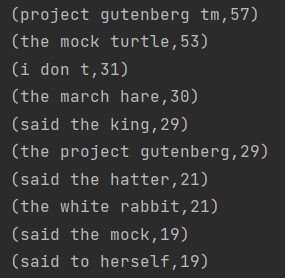
\includegraphics[height=7cm]{captures/primeraPart/ngrames/execucio.jpg}
			\end{center}
		
		\subsubsection{Vector space model}
		
			\begin{itemize}
			
				\item Resultat execució (\textbf{n = 0}):
			
				\begin{center}
					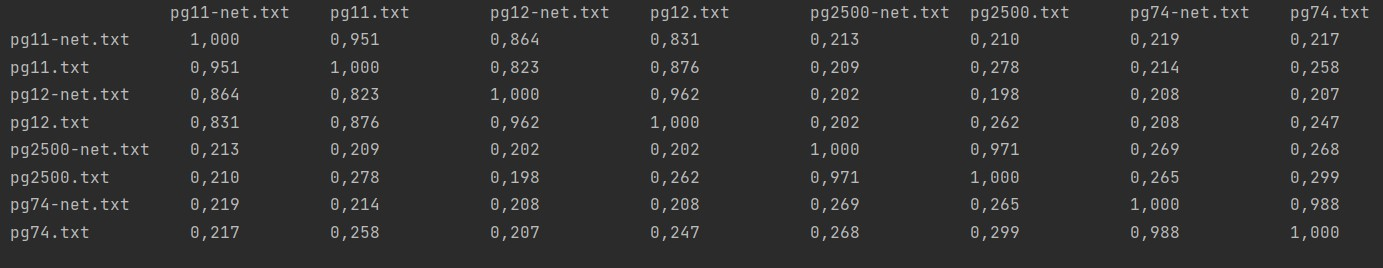
\includegraphics[height=3cm]{captures/primeraPart/vectorspacemodel/execucio0.jpg}
				\end{center}
				
				\item Resultat execució (\textbf{n = 2}):
				
				\begin{center}
					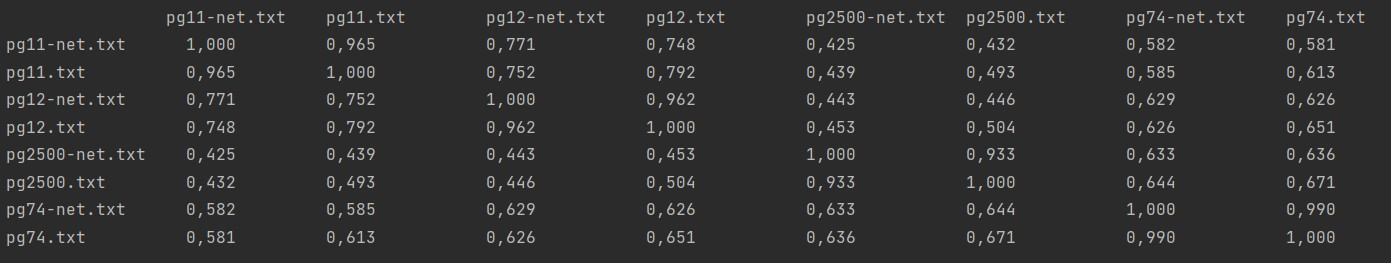
\includegraphics[height=3cm]{captures/primeraPart/vectorspacemodel/execucio2.jpg}
				\end{center}
				
				\item Resultat execució (\textbf{n = 3}):
				
				\begin{center}
					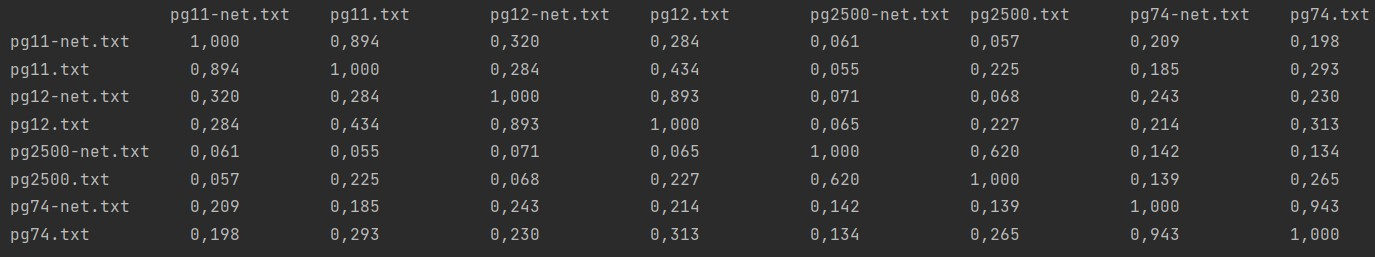
\includegraphics[height=3cm]{captures/primeraPart/vectorspacemodel/execucio3.jpg}
				\end{center}	
			
			\end{itemize}
			
	\subsection{Resultats Execucions Segona Part}
	
		\begin{itemie}
			\item \textbf{1000}:
			
			\item \textbf{5000}:
		\end{itemize}


% Secció: Taula de rendiment
\section{Taula de rendiment}

	Per la realització de les diferents proves, s'ha utilitzat l'equip amb les següents especificacions.

	\subsection{Especificacions}
		
		\begin{center}
			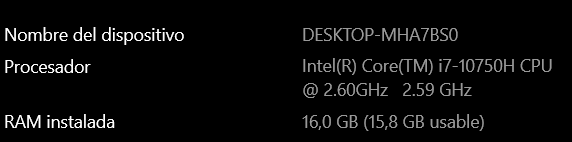
\includegraphics[height=4cm]{captures/especificacionsEquip/especificacions1.png}
		\end{center}
		
		\begin{center}
			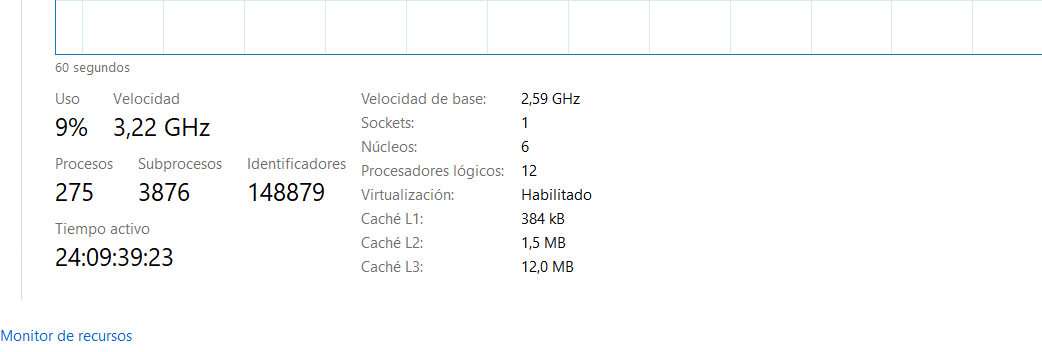
\includegraphics[height=5cm]{captures/especificacionsEquip/especificacions2.png}
		\end{center}
		
	\subsection{Taula dels actors}
	
		Les proves s'han realitzat amb tots els fitxers disponibles, i la taula representa per cada número d'actors, quants segons triga.
	
		\begin{table}[h!]
			\centering
			\begin{tabular}{||c c c c||} 
			 \hline
			 \multicolumn{4}{|c|}{Número d'actors} \\
			 \hline
			 1 & 4 & 10 & 20 \\ [0.5ex] 
			 \hline
			  0.5 & 0.5 & 0.5 & 0.5 \\ [1ex] 
			 \hline
			\end{tabular}
		\end{table}

% Secció: Altres consideracions
\section{Alltres consideracions}

Com s'indiquen a les proves anteriors, s'han realitzat amb tots els fitxers disponibles i s'ha aconseguit un molt bon temps. Per tant, molt contents amb el resultat final.


\end{document}


